\section{Ergebnisse}
\subsection{Portfoliodatensatz}
Die Erzeugung eines realitätsnahen Datensatzes ist ein wesentlicher Schritt in dieser Forschung, da nur dadurch die Quantifizierung physischer und Transitionsrisiken im Hypothekenportfolio ermöglicht wird. Nach Abschluss aller in Kapitel \ref{sec:createportfolio} beschriebenen Schritte wurde ein realistisches Portfolio von Hypotheken-Immobilien erstellt.
Abbildung \ref{fig:hypothekenportfolio} zeigt die resultierende Distribution der Datenpunkte auf der Karte Bayerns.

\begin{figure}[htbp]
    \centering
    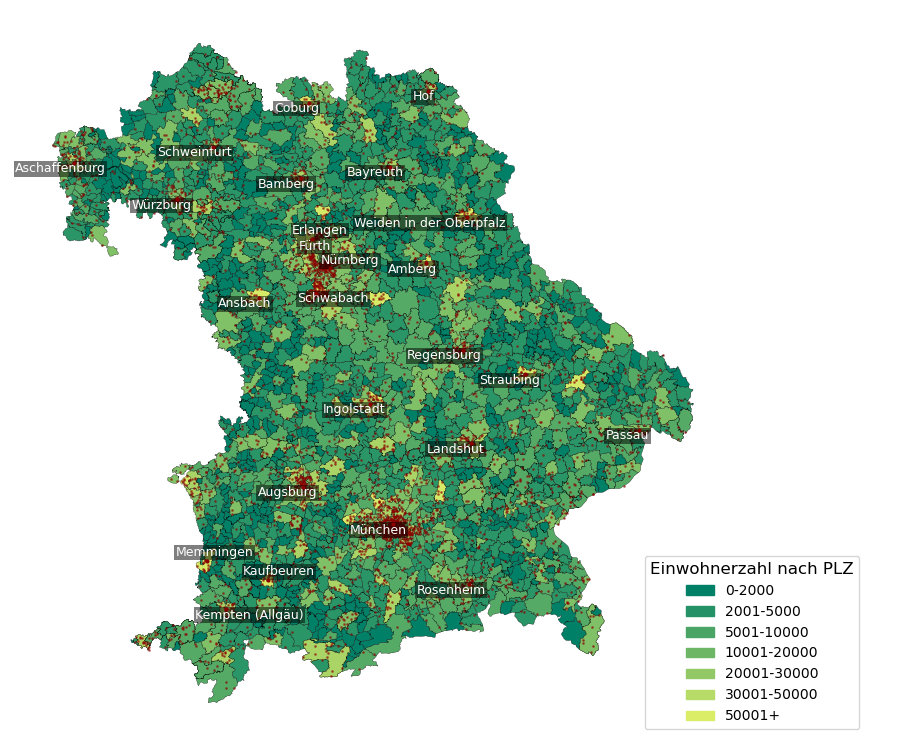
\includegraphics[width=1.2\textwidth]{figures/bayern_por_pop.png} 
    \caption{Datenpunktverteilung im Hypothekenportfolio Bayern. Quelle: Eigene Darstellung}
    \label{fig:hypothekenportfolio}
\end{figure}
\FloatBarrier

Abbildung \ref{fig:bayernflut} präsentiert das Resultat dieser Vereinheitlichung der Datenpunkte auf der Karte Bayerns mit den Hochwasserrisikogebieten.

\begin{figure}[htbp]
    \centering
    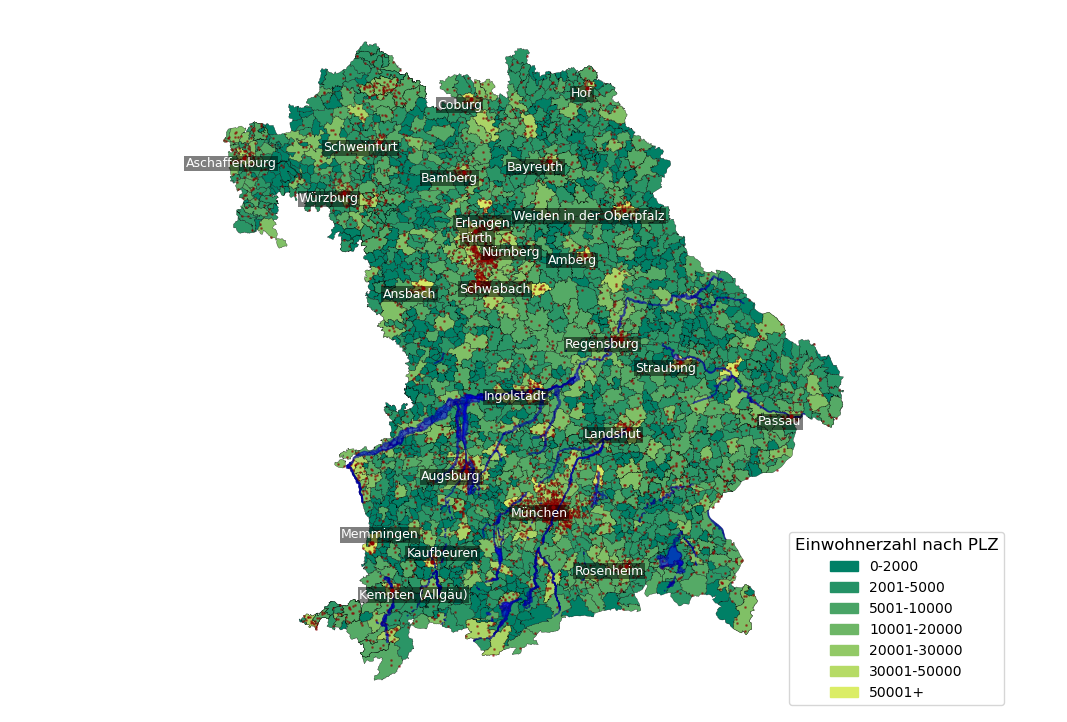
\includegraphics[width=1.2\textwidth]{figures/bayern_flut.png} 
    \caption{Visualisierung historischer Hochwasserereignisgebiete und Verteilung des Darlehensportfolios in Bayern. Quelle: Eigene Darstellung}
    \label{fig:bayernflut}
\end{figure}
\FloatBarrier

Als Ergebnis entstand ein umfassender Datensatz, dessen Grundlage die in Tabelle \ref{tab:objekt-variablen} beschriebenen Objektvariablen bilden.
\begin{table}[htbp]
    \centering
    \small
    \caption{Übersicht über das Hypothekenportfolio und die relevanten Objekt-Variablen}
    \label{tab:objekt-variablen}
    \begin{tabularx}{1.0\textwidth}{>{\raggedright\arraybackslash}X >{\raggedright\arraybackslash}X}
        \toprule
        \textbf{Objekt-Variablen} & \textbf{Erklärung} \\
        \midrule
        ID & Identifikationsnummer \\
        \addlinespace
        Ort & Ort der Immobilie \\
        \addlinespace
        Landkreis & Landkreis der Immobilie \\
        \addlinespace
        Latitude & Breitengrad der Immobilie zur genauen Lokalisierung \\
        \addlinespace
        Longitude & Längengrad der Immobilie zur genauen Lokalisierung \\
        \addlinespace
        GEB\_Q & Hochwasser Ergebnis \\
        \addlinespace
        AEP & Jährliche Überschreitungswahrscheinlichkeit \\
        \addlinespace
        Überschwemmung Tiefe & Tiefe der Überschwemmung an dem Punkt \\
        \addlinespace
        Überschwemmungsrisiko Stufe & Stufe des Überschwemmungsrisikos \\
        \addlinespace
        Energieklasse & Energieeffizienzklasse der Immobilie \\
        \addlinespace
        Quadratmeterpreise & Preis pro Quadratmeter der Immobilie \\
        \addlinespace
        Wohnfläche & Gesamte Wohnfläche der Immobilie in Quadratmetern \\
        \addlinespace
        Aktueller Immobilienwert & Der aktuelle Wert der Immobilie \\
        \addlinespace        Aktuelles LTV & Aktuelles Verhältnis von Darlehen zu Wert (Loan-to-Value) \\
        \bottomrule
    \end{tabularx}
\end{table}
\FloatBarrier
Der Datensatz umfasst 3853 Datenpunkte, verteilt auf 1522 Orte und 71 Landkreise in Bayern. Diese Verteilung ist plausibel und entspricht den Annahmen basierend auf der bayerischen Bevölkerungsdichte. Die Verteilung der Energieklassen der Datenpunkte stimmt mit der bayerischen Energieklassenverteilung laut Tabelle \ref{tab:epc_bayern} überein. Ähnlich orientiert sich die LtV-Verteilung an Tabelle \ref{tab:beleihungsauslauf2023}.
\begin{table}[htbp]
    \centering
    \caption{Statistische Zusammenfassung der Hypothekendaten}
    \label{tab:hypothekenuberblick}
    \small
    \begin{tabularx}{\textwidth}{>{\raggedright\arraybackslash}m{3.5cm}*{5}{>{\centering\arraybackslash}X}}
    \toprule
    Metrik & Mean & Median & Min & Max & Std \\
    \midrule
    Preis/m² & 2.458,57 & 2.032,01 & 685,48 & 5.297,69 & 1.320,59 \\
    Wohnfläche & 114,40 & 111,78 & 80,00 & 168,23 & 29,14 \\
    Akt. Immnwert & 281.726,31 & 229.186,05 & 54.838,79 & 889.649,95 & 173.681,59 \\
    Akt. LtV & 0,5978 & 0,6000 & 0,4200 & 0,7500 & 0,1012 \\
    Darlehenbetrag & 168.148,10 & 136.034,00 & 26.368,90 & 662.763,36 & 108.638,21 \\
    \bottomrule
    \end{tabularx}
\end{table}

\subsection{Physische Risiko}
Die Hochwasserrisikostufen im erstellten Portfolio sind wie folgt verteilt: 1 hohes, 17 mittlere, 12 niedrige und 3823 sehr niedrige Risiken. Diese Risikostufeverteilung wird in Abbildung \ref{fig:riskostufe} graphisch dargestellt und visualisiert.
\begin{figure}[htbp]
    \centering
    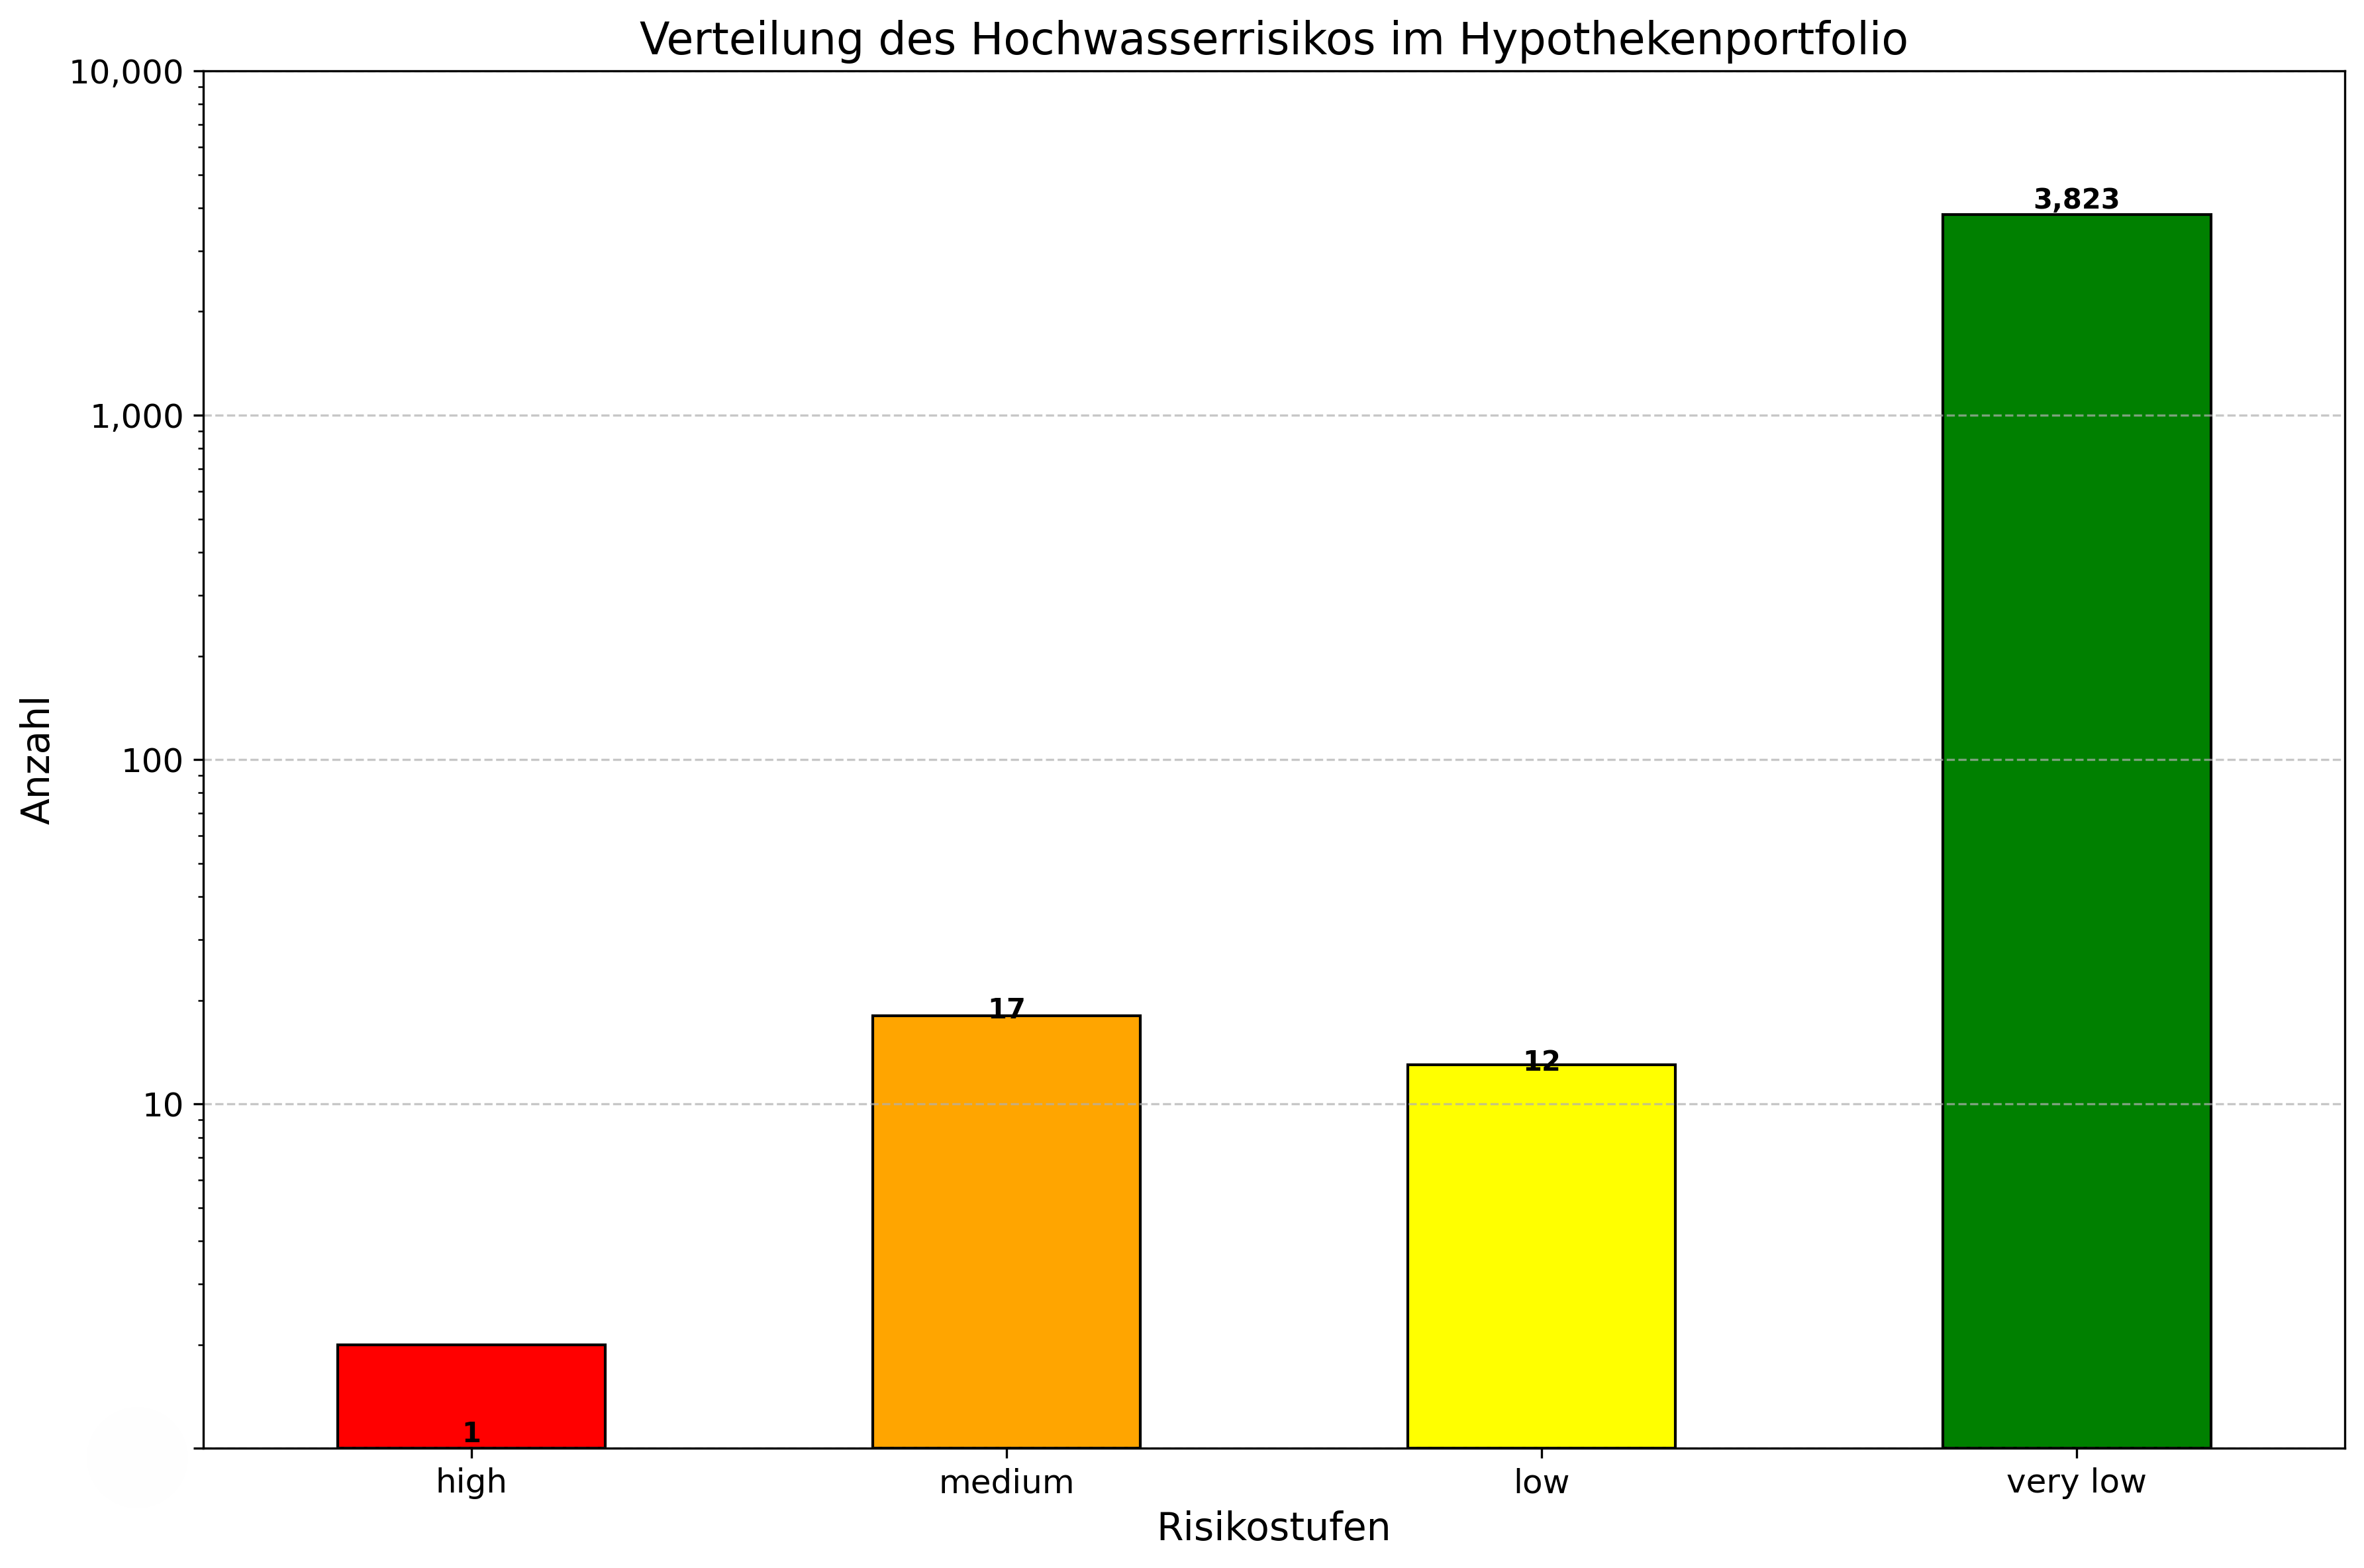
\includegraphics[width=0.8\textwidth]{figures/hochwasserrisiko_verteilung.png}
    \caption{Verteilung der Hochwasserrisikostufen im Hypothekenportfolio. Quelle: Eigene Darstellung}
    \label{fig:riskostufe}
\end{figure}
\FloatBarrier
Mittels des digitalen Geländemodells von Bayerns sowie Pegelnullpunkt und Hochwasserstand von \textcite{bayern2016hochwassernachrichtendienst} wurde die Überflutungstiefe bestimmt. Dies betrifft Datenpunkte in den Kategorien hoch, mittel und niedrig.

Nach der Berechnung der Überflutungstiefe kann durch den Vergleich mit der Schadenfunktion in Abbildung \ref{fig:damage_curve2} der entsprechende Schadensfaktor ermittelt werden. Basierend auf diesem Schadensfaktor lässt sich mithilfe der Gleichung \ref{eq:schaden} der Immobilienschaden quantifizieren. Die Resultate dieser Berechnungen für den Immobilienschaden werden anschließend in Abbildung \ref{fig:schadenwert} grafisch dargestellt.
\begin{figure}[htbp]
    \centering
    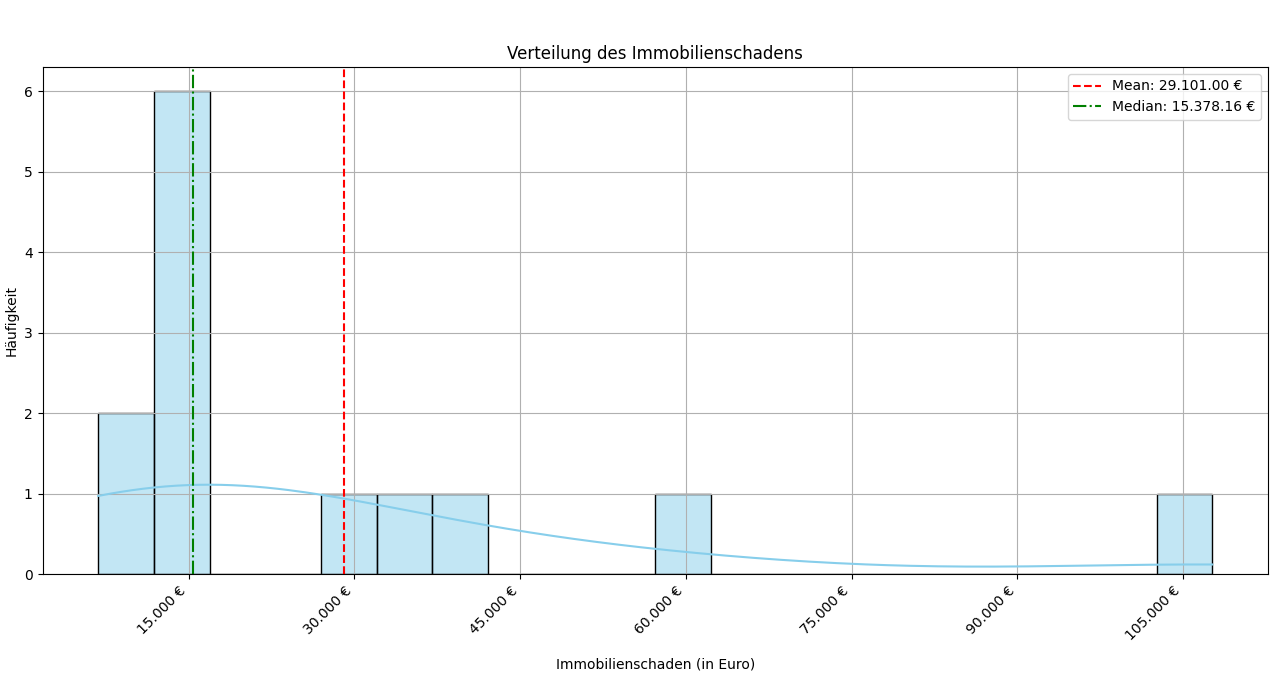
\includegraphics[width=\textwidth]{figures/flutschaden.png}
    \caption{Verteilung des Immobilienschaden im Hypothekenportfolio. Quelle: Eigene Darstellung}
    \label{fig:schadenwert}
\end{figure}
\FloatBarrier
In der folgenden Abbildung \ref{fig:schadenereignis} wird der prozentuale Gesamtschadenwert im Vergleich zum Gesamtimmobilienwert im Falle des Eintritts eines Schadensereignisses dargestellt. Abbildung \ref{fig:schadenereignis_jahr} zeigt den prozentualen Gesamtschadenwert im Vergleich zum Gesamtimmobilienwert, wenn ein Schadensereignis innerhalb eines Jahres eintritt.\begin{figure}[H]
    \centering
    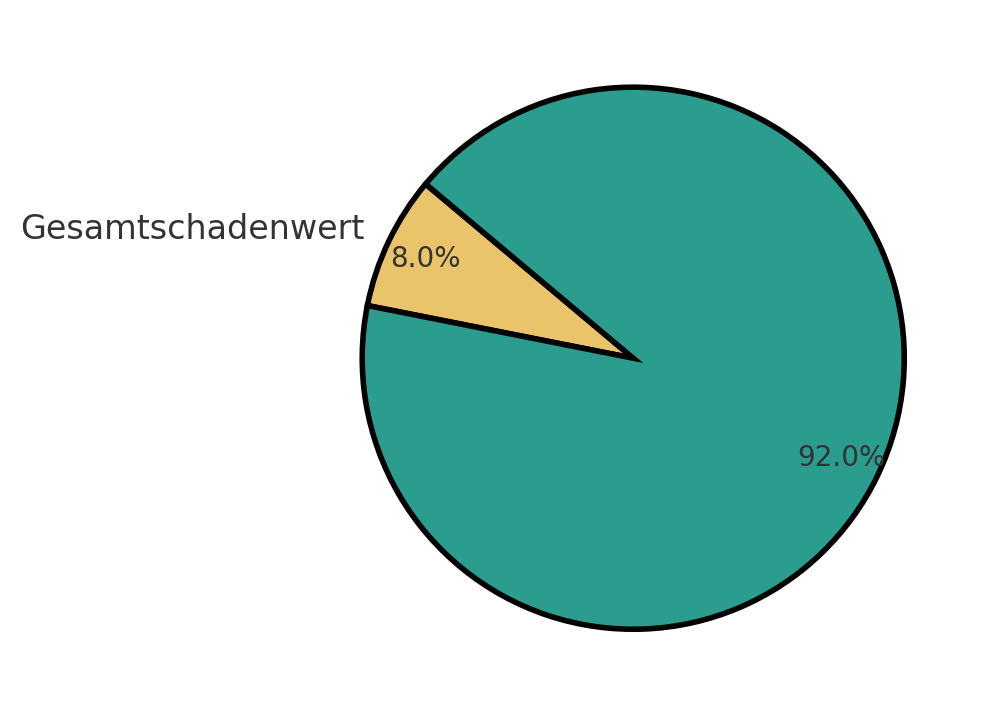
\includegraphics[width=0.45\textwidth]{figures/roundchartsloss.png}
    \caption{Prozentualer Gesamtschaden am Immobilienwert im Schadensfall}
    \label{fig:schadenereignis}
\end{figure}

\begin{figure}[H]
    \centering
    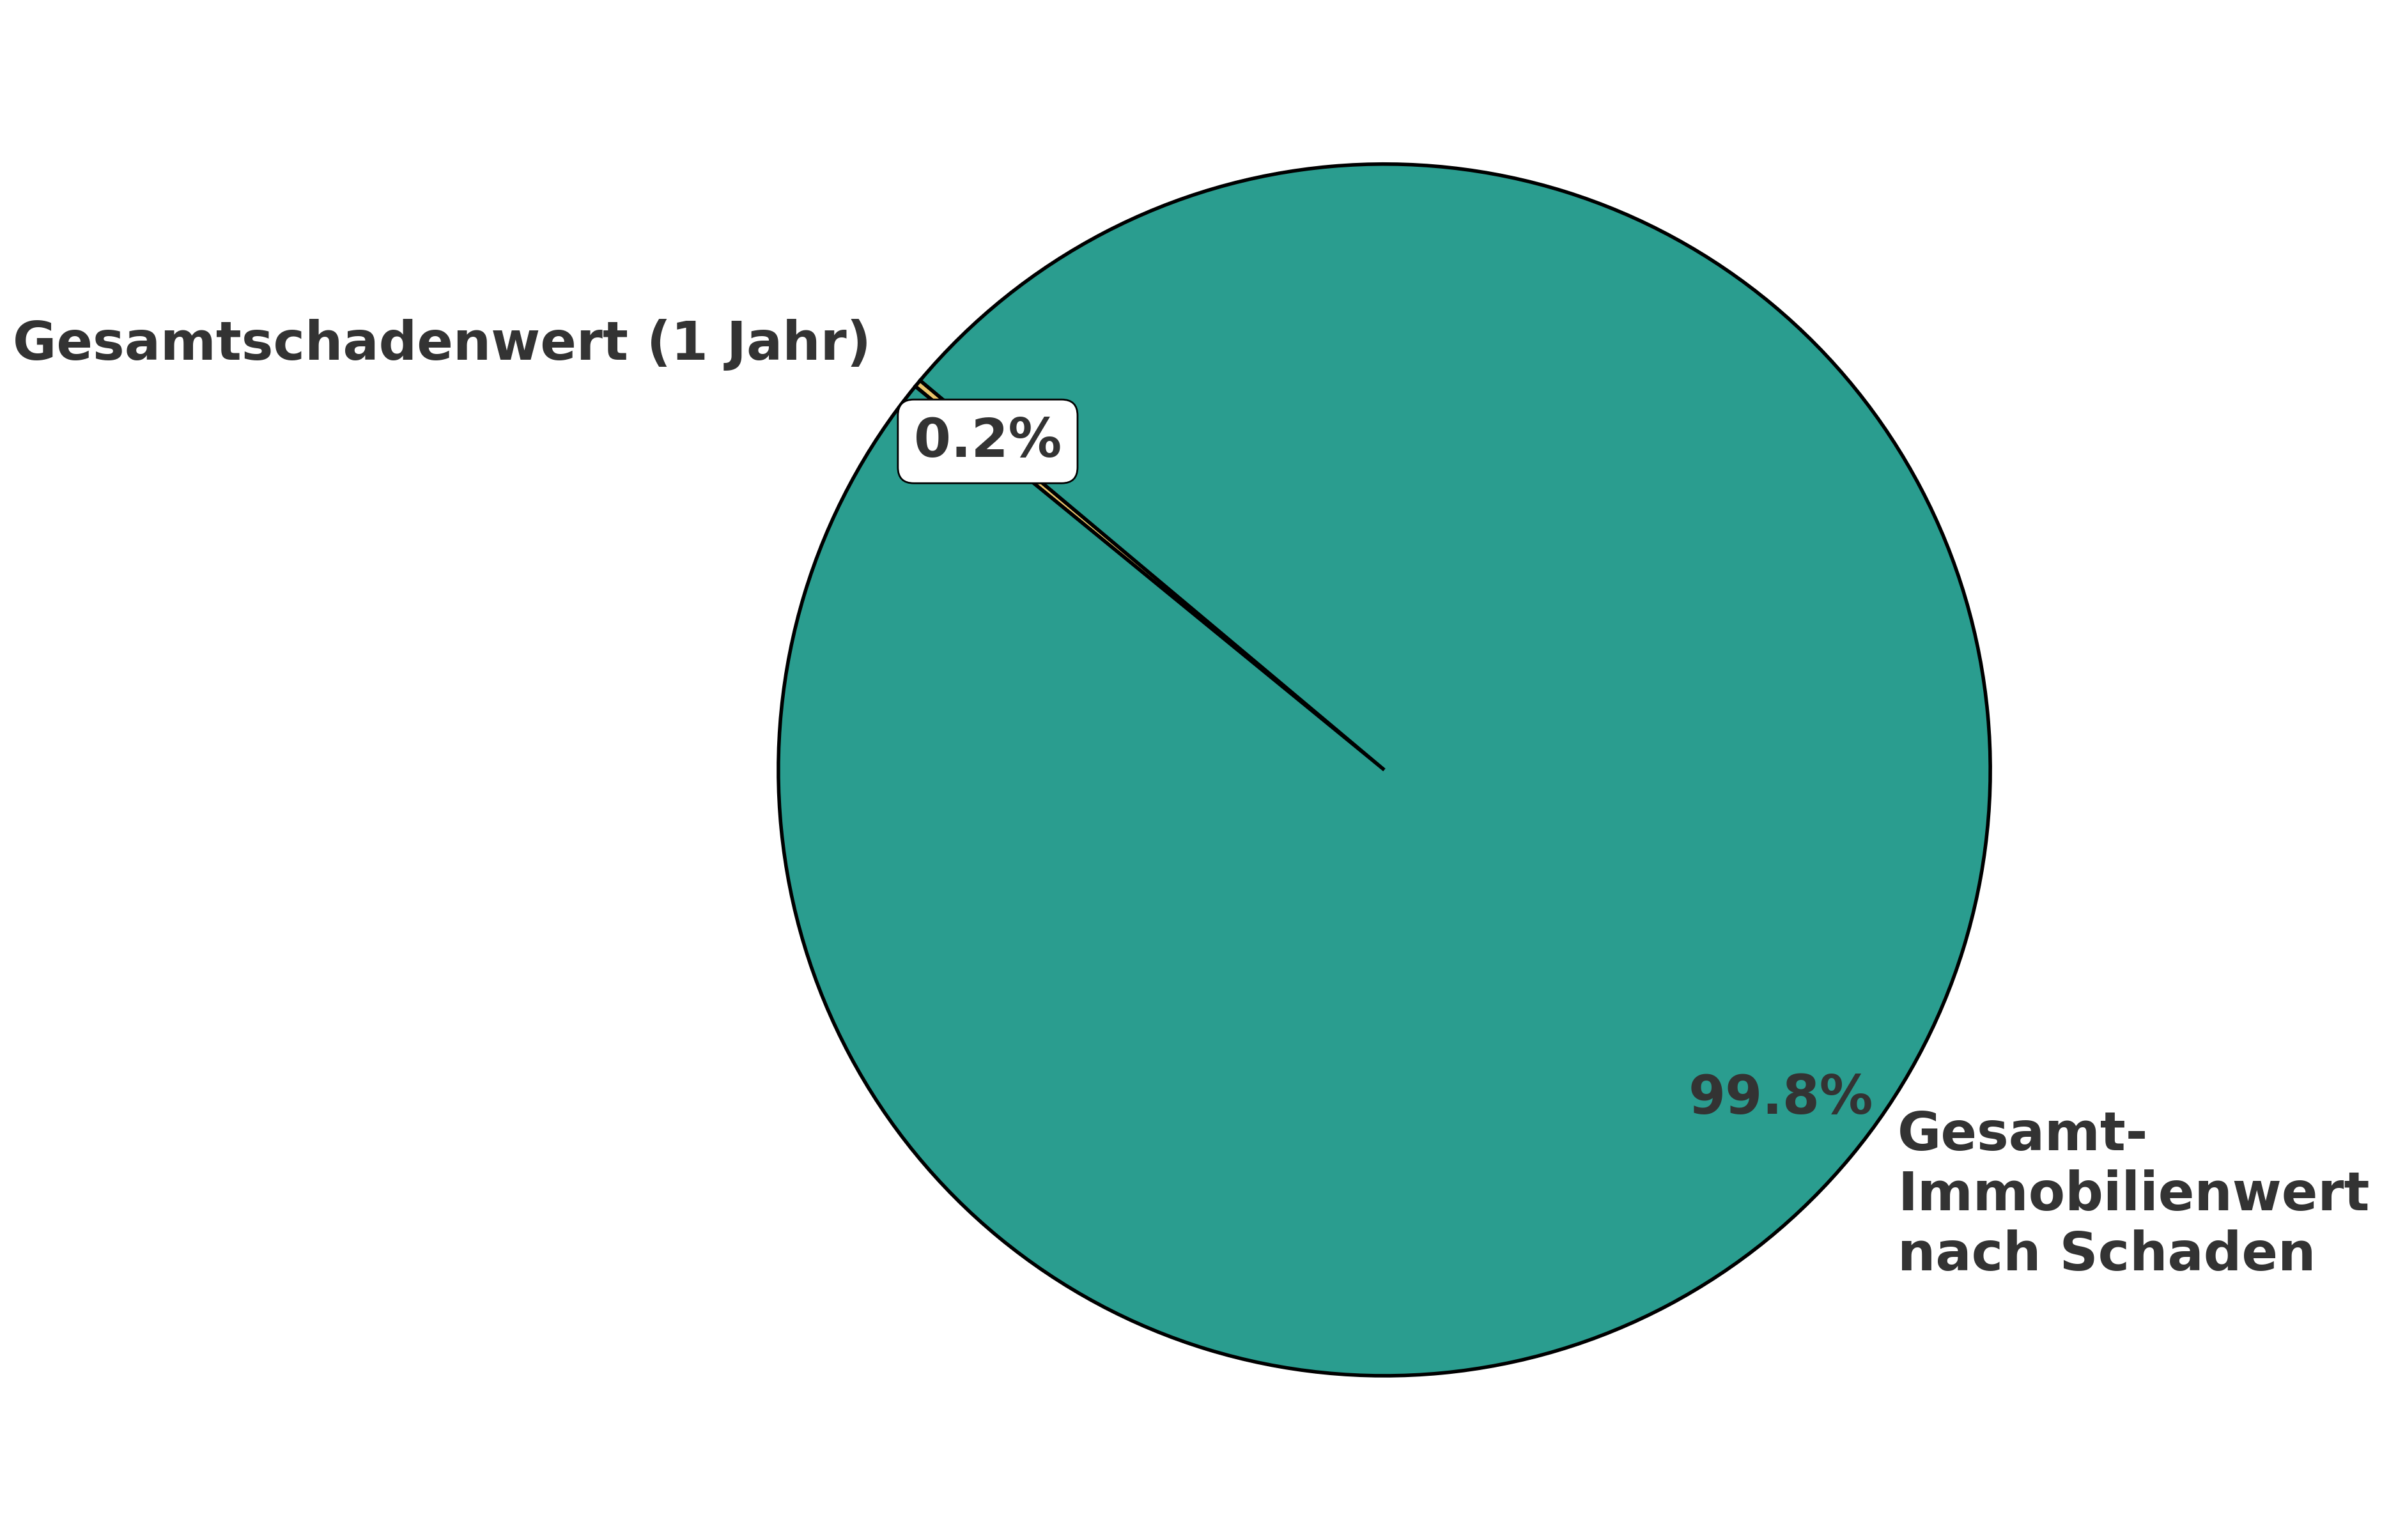
\includegraphics[width=0.45\textwidth]{figures/roundchartloss1year.png}
    \caption{Prozentualer Gesamtschaden am Immobilienwert im Jahresschadensfall}
    \label{fig:schadenereignis_jahr}
\end{figure}


Abbildung \ref{fig:schadenLtV} vergleicht den aktuellen Beleihungsauslauf mit dem Beleihungsauslauf nach Eintritt eines Schadensereignisses.

\begin{figure}[htbp]
    \centering
    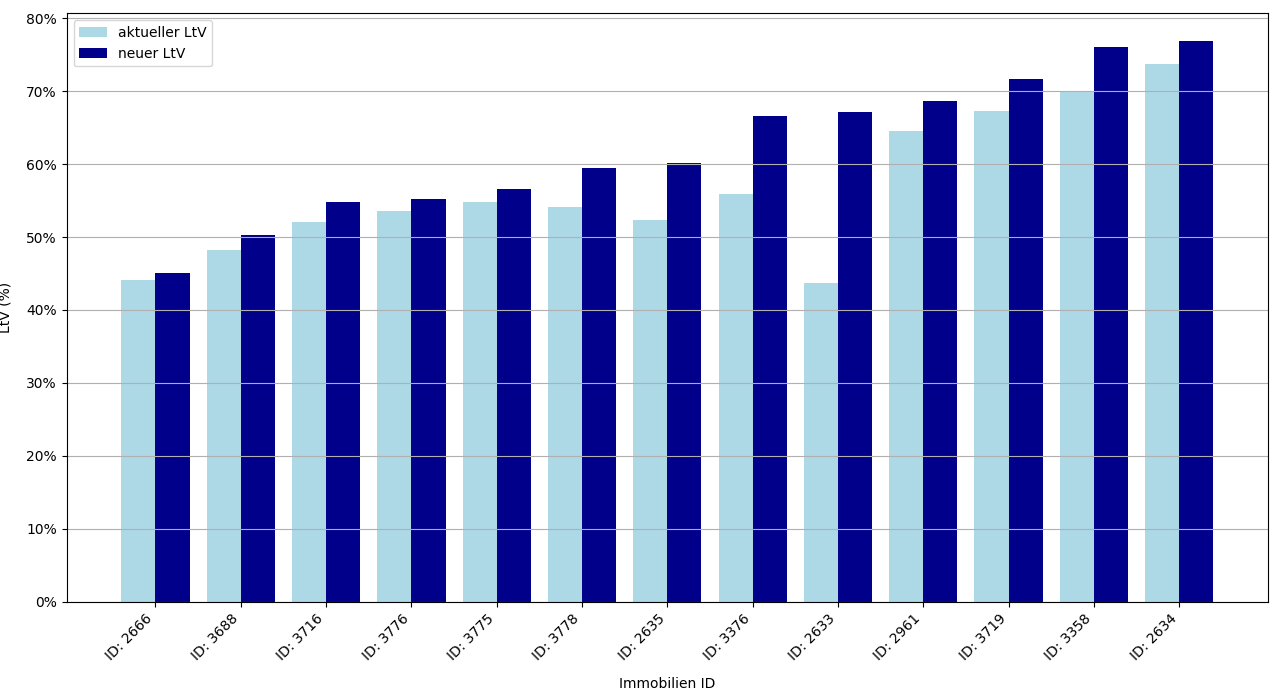
\includegraphics[width=0.5\textwidth]{figures/compareltv.png}
    \caption{Vergleich des aktuellen und neuen Beleihungsauslaufs nach Schadenseintritt. Quelle: Eigene Darstellung}
    \label{fig:schadenLtV}
\end{figure}
\FloatBarrier



\subsection{Transitionsrisiko}
Abbildung \ref{fig:endpreis_energie} zeigt das Ergebnis der Berechnungen des Endpreises für Energie, basierend auf den NGFS-Szenarien, unter Berücksichtigung der Mehrwert- und Energiesteuern in vier NGFS-Szenarien: Netto-Null, Ungeordnet (Disorderly), Unter 2°C (Below 2 Degrees) und Aktuelle Richtlinien (Current Policies).

\begin{figure}[htbp]
    \centering
    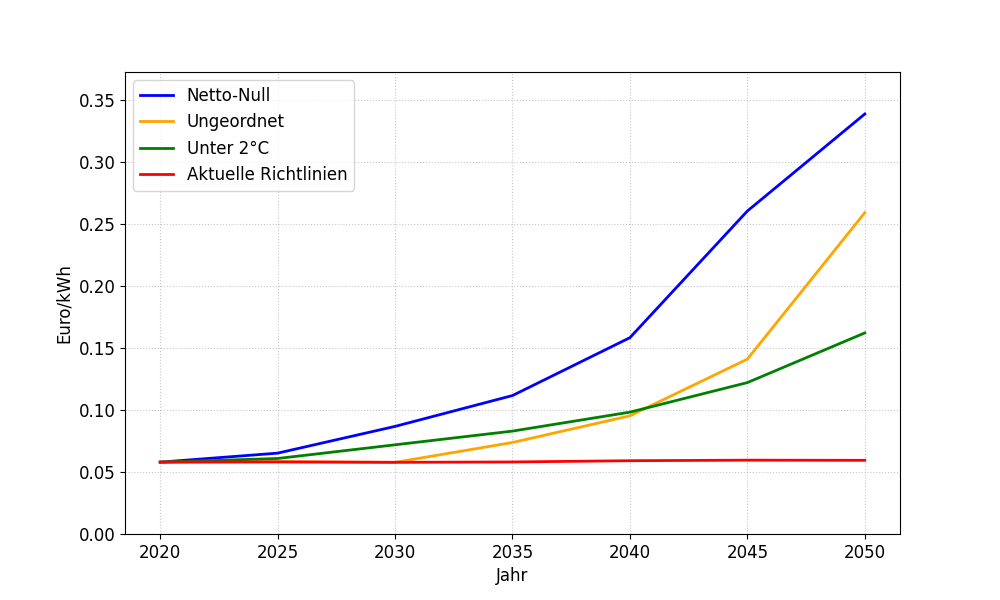
\includegraphics[width=\textwidth]{figures/endpreis.png}
    \caption{Endpreis der Energie mit Mehrwert- und CO2-Steuern nach NGFS-Szenarien. Quelle: Eigene Darstellung}
    \label{fig:endpreis_energie}
\end{figure}
\FloatBarrier

Auf Grundlage des zuvor berechneten Endenergiepreises und der Formel aus Abschnitt \ref{sec:endenfkt} wurde die absolute Wertänderung der Immobilien ermittelt. Diese Berechnungen wurden für Häuser mit Energieeffizienzklassen unterhalb von A und A+ vorgenommen. Die Analysen ergaben Daten zur jährlichen absoluten Werteentwicklung dieser Immobilien. Zudem wurden verschiedene Szenarien betrachtet.und der Formel aus Abschnitt \ref{sec:endenfkt} wurde die absolute Wertänderung der Immobilien ermittelt. Diese Berechnungen wurden für Häuser mit Energieeffizienzklassen unterhalb von A und A+ vorgenommen. Die Analysen ergaben Daten zur jährlichen absoluten Werteentwicklung dieser Immobilien. Zudem wurden verschiedene Szenarien betrachtet.

Die folgenden Abbildungen zeigen die absoluten Immobilien-Wertsveränderungen in Abhängigkeit von Zeit und Szenario.
% Stellen Sie sicher, dass dies im Hauptteil Ihres Dokuments ist
\begin{figure}[htbp]
    \centering
    \begin{subfigure}[b]{0.48\textwidth}
        \centering
        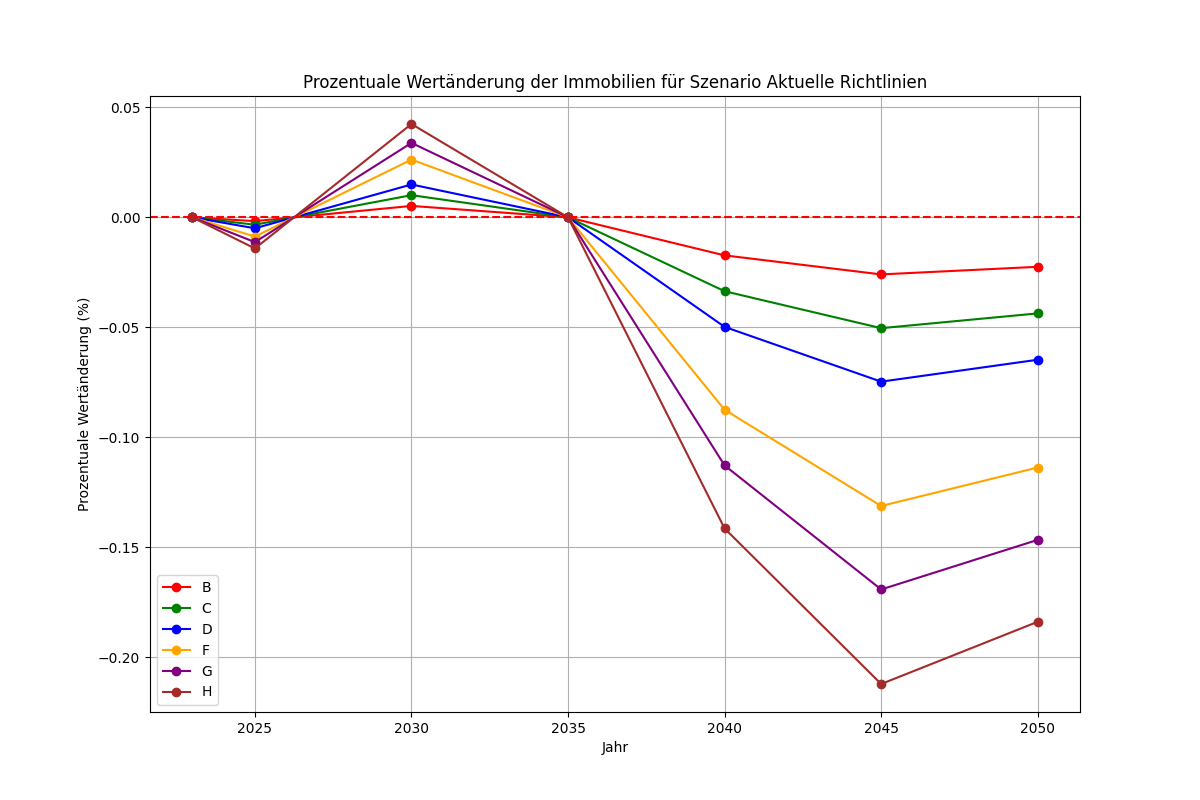
\includegraphics[width=\textwidth]{figures/Aktuelle Richtlinien_percentage_change_plot.png}
        \caption{Prozentuale Wertänderung der Immobilien im Szenario Aktuelle Richtlinien.}
        \label{fig:aktuelle_richtlinien}
    \end{subfigure}
    \hfill
    \begin{subfigure}[b]{0.48\textwidth}
        \centering
        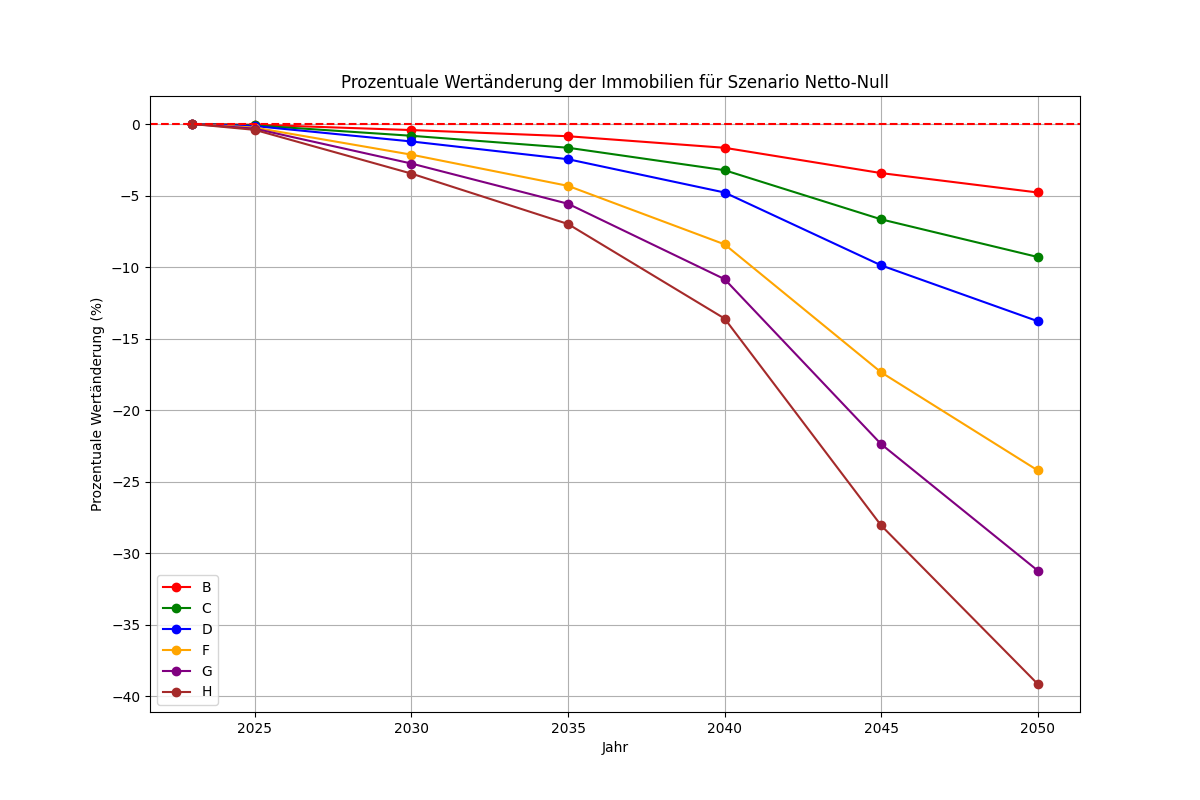
\includegraphics[width=\textwidth]{figures/Netto-Null_percentage_change_plot.png}
        \caption{Prozentuale Wertänderung der Immobilien im Szenario Netto-Null.}
        \label{fig:netto_null}
    \end{subfigure}
    
    \vspace{1em}
    
    \begin{subfigure}[b]{0.48\textwidth}
        \centering
        \includegraphics[width=\textwidth]{figures/Unter 2°C_percentage_change_plot.png}
        \caption{Prozentuale Wertänderung der Immobilien im Szenario Unter 2°C.}
        \label{fig:unter_2c}
    \end{subfigure}
    \hfill
    \begin{subfigure}[b]{0.48\textwidth}
        \centering
        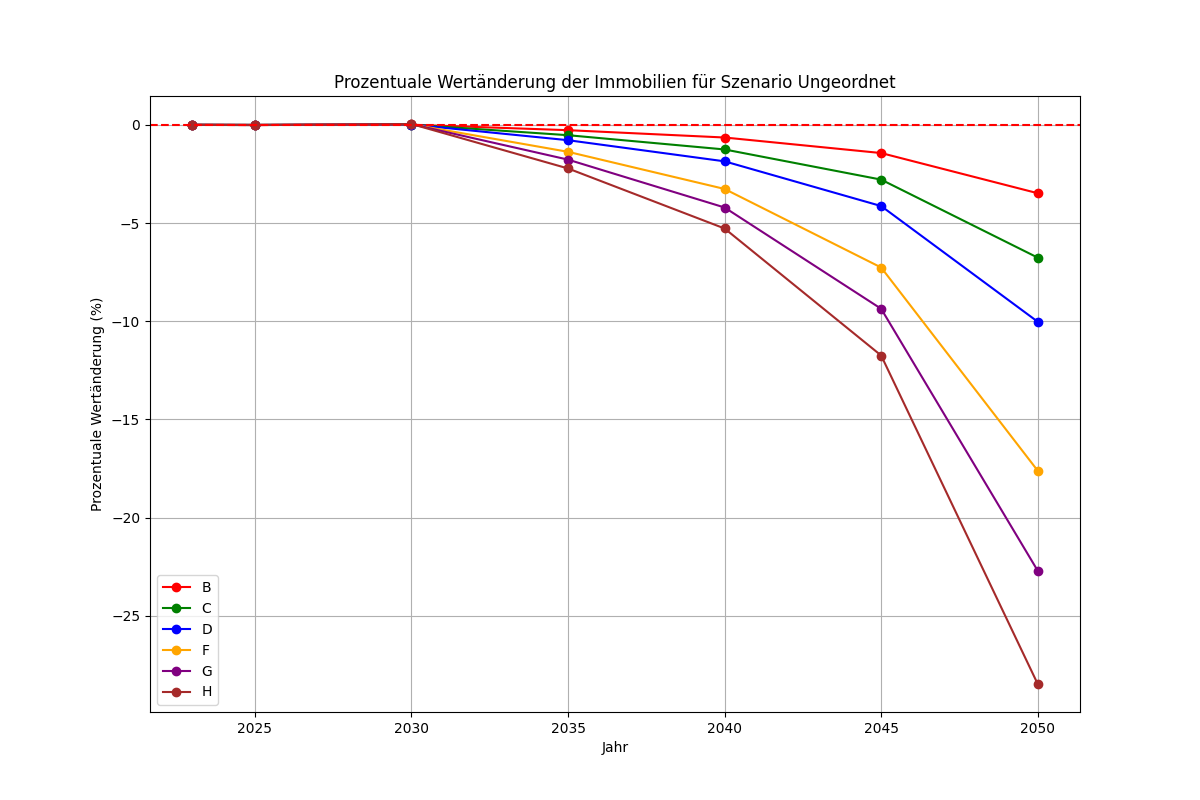
\includegraphics[width=\textwidth]{figures/Ungeordnet_percentage_change_plot.png}
        \caption{Prozentuale Wertänderung der Immobilien im Szenario Ungeordnet.}
        \label{fig:ungeordnet}
    \end{subfigure}
    \caption{Prozentuale Wertänderung der Immobilien in verschiedenen Szenarien.}
    \label{fig:all_scenarios}
\end{figure}